\begin{frame}{$d(K^-, n)\pi^{\mp}\Sigma^{\pm}"$ 断面積}
  \label{page:piS_CS}
  
  \tminipageTwo{
    \begin{figure}
      $d(K^-, n)"\pi^{\mp}\Sigma^{\pm}$のアクセプタンス
      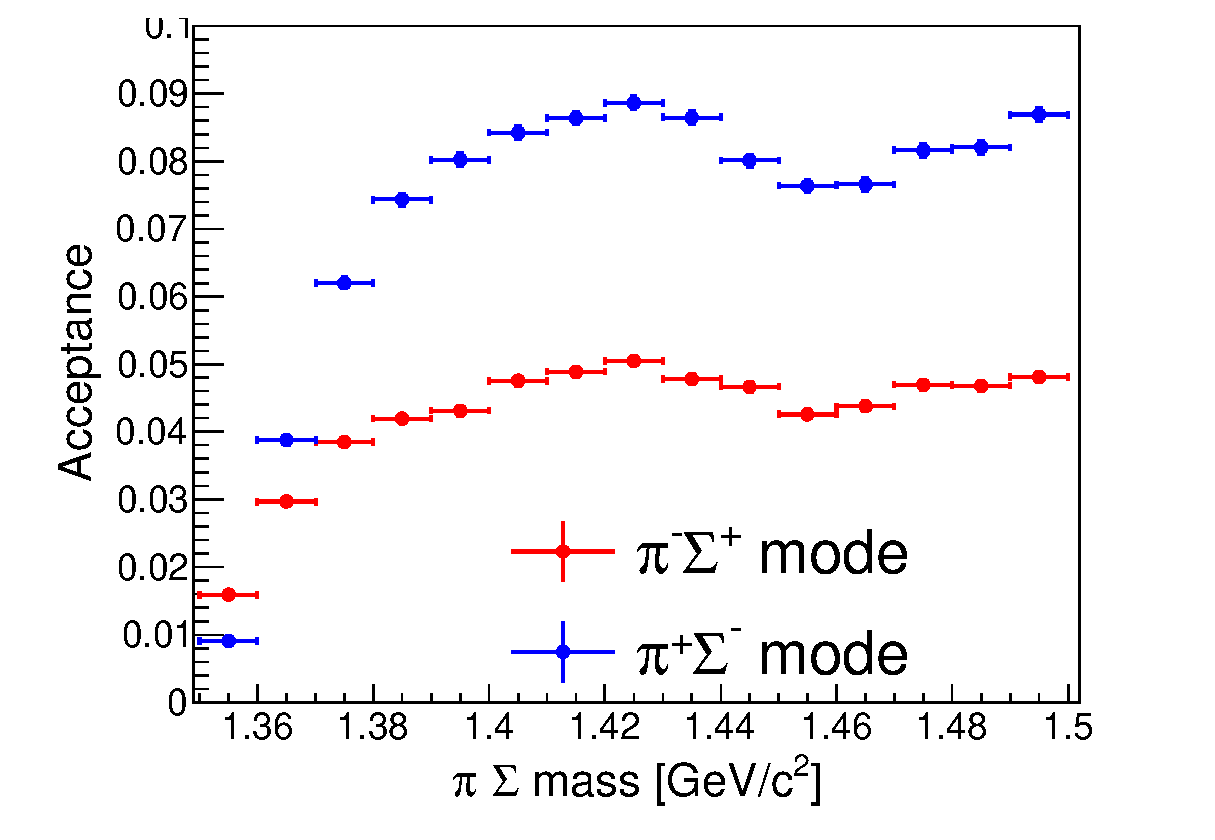
\includegraphics[width=4.5cm]{../pic/Run78/KN_ana_NC170_2sigma/kn_acc.eps}
    \end{figure}
    \vspace{-5mm}
    \centering
    \scriptsize
    データ解析と同じ解析ルーチンを用いた\\
    CDSの解析効率を含むアクセプタンス。

    \tiny
    %%    \begin{table}
  \begin{tabular}{ |c|c|c|c| }
    \hline
    項目           &  値                & エラー  & エラー(割合)\\
    \hline
    ルミノシティー &  $5.162\times10^3$ & $0.014\times10^3$  & 2.6\% \\
    NC(System)検出効率     & 0.291      & 0.016 & 5.0\% \\
    CDC検出効率            & 0.977      & 0.004 & 0.41\%\\
    \hline
    \hline
    合計                   &            &       & 5.65\% \\
    \hline
  \end{tabular}
\end{table}
  

    \begin{table}
      \begin{tabular}{ |c|c|c|c| }
        \hline
        項目           &  値                & エラー  & 割合)\\
        \hline
        ルミノシティー &  $5.162\times10^3$ & $0.014\times10^3$  & 2.6\% \\
        NC検出効率     & 0.291      & 0.016 & 5.0\% \\
        CDC検出効率            & 0.977      & 0.004 & 0.41\%\\
        \hline
        \hline
        合計                   &            &       & 5.65\% \\
        \hline
      \end{tabular}
    \end{table}
    \vspace{-3mm}
    NC検出効率はCVC/BVCのオーバーキルを含む
  }{
    \begin{figure}
      $d(K^-, n)"\pi^{\mp}\Sigma^{\pm}$の断面積
      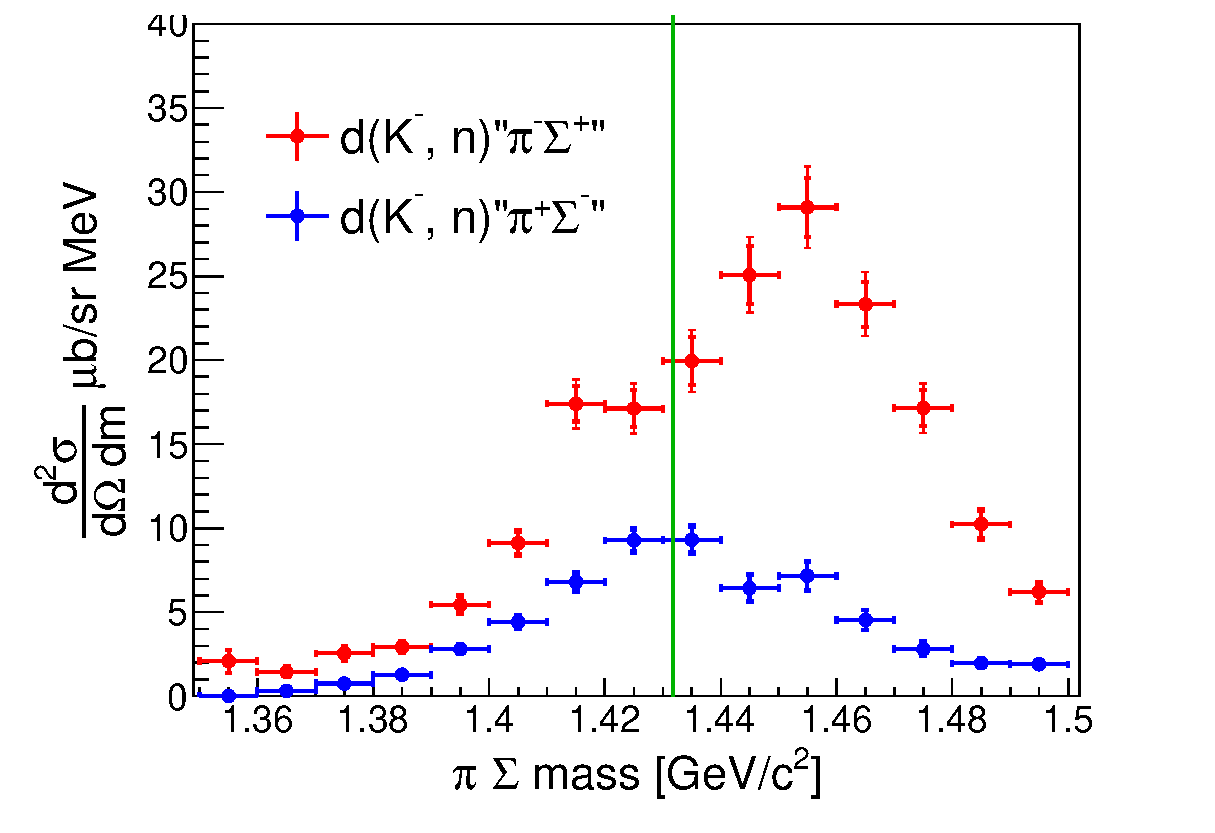
\includegraphics[width=6.5cm]{../pic/Run78/KN_ana_NC170_2sigma/pimSp_pipSm_CS.eps}
    \end{figure}
    \vspace{-5mm}
    \centering
    \scriptsize
    内側のBoxは統計エラーを外側のBoxは\\
    フィッティングエラーを含むエラーを、\\
    エラーバーはスケールファクター[左表]\\
    を含むエラーを表す。\\
    各エラーは自乗平均で計算。\\
  }
\end{frame}
